\chapter{Related Work}
\label{ch:related_work}
\glsresetall
Having established a certain understanding of the core concepts that are used throughout this thesis, this chapter presents the reader with an overview of work related to the present research. That is to say: research that has to do with \gls{kd} applied to Transformer(-based) architectures.

In and on itself, \gls{kd} as described by \citet{hinton2015distilling} provides only a general recipe that leaves much to be specified, such as:
\begin{fullwidth}
\begin{itemize}
    \item What (ensemble of) teacher (and student) network architecture(s) do you use?
    \item What transfer dataset do you use?
    \item What composition of the combined loss function (see \cref{eq:combined_kd_loss}) do you use?
\end{itemize}
\end{fullwidth}

While this provides already plenty degrees of freedom, when it comes to Transformer(-based) architectures specifically, at least one more important variable can be added to the mix:
\begin{fullwidth}
\begin{itemize}
    \item At what stage (pre-training, fine-tuning or both) is \gls{kd} applied?
\end{itemize}
\end{fullwidth}

The last variable to consider is more generally applicable to all scientific research:
\begin{fullwidth}
\begin{itemize}
    \item How do you evaluate your approach / method?
\end{itemize}
\end{fullwidth}

As there are (too) many possible categorizations possible along the aforementioned dimensions, this chapter presents the related works chronologically, instead, by date of (pre-)publication. This does mean that, unlike the other chapters in this thesis, the current chapter lacks structure with sections and subsections and soforth. Despite this, it should still be a clear read.


% tang 2019
To the best of our knowledge, \citet{tang2019distilling} were the first to apply (a form of) \gls{kd} to BERT. Specifically, they applied \gls{kd} on the end-task level for three different end-tasks (SST-2, MNLI and QQP, a subset of the \gls{glue} benchmark, see \cref{subsec:GLUE}). For each end-task, they used \bertlarge fine-tuned on that specific end-task as their teacher network, and a single-layer \gls{bilstm} \citep{hochreiter1997long} as their student network for single-sentence tasks, 
% as illustrated in \cref{fig:BiLSTM_tang_2019}, 
and its siamese counter part for sentence-pair tasks.
% \sidenote{Teacher network: \bertlarge\\Student network: \gls{bilstm}\\Transfer dataset: fine-tuning task (GLUE)\\Loss function: linear combination of \gls{ce} (hard) and \gls{mse} (soft)\\Stage: fine-tuning}

% \begin{marginfigure}
%     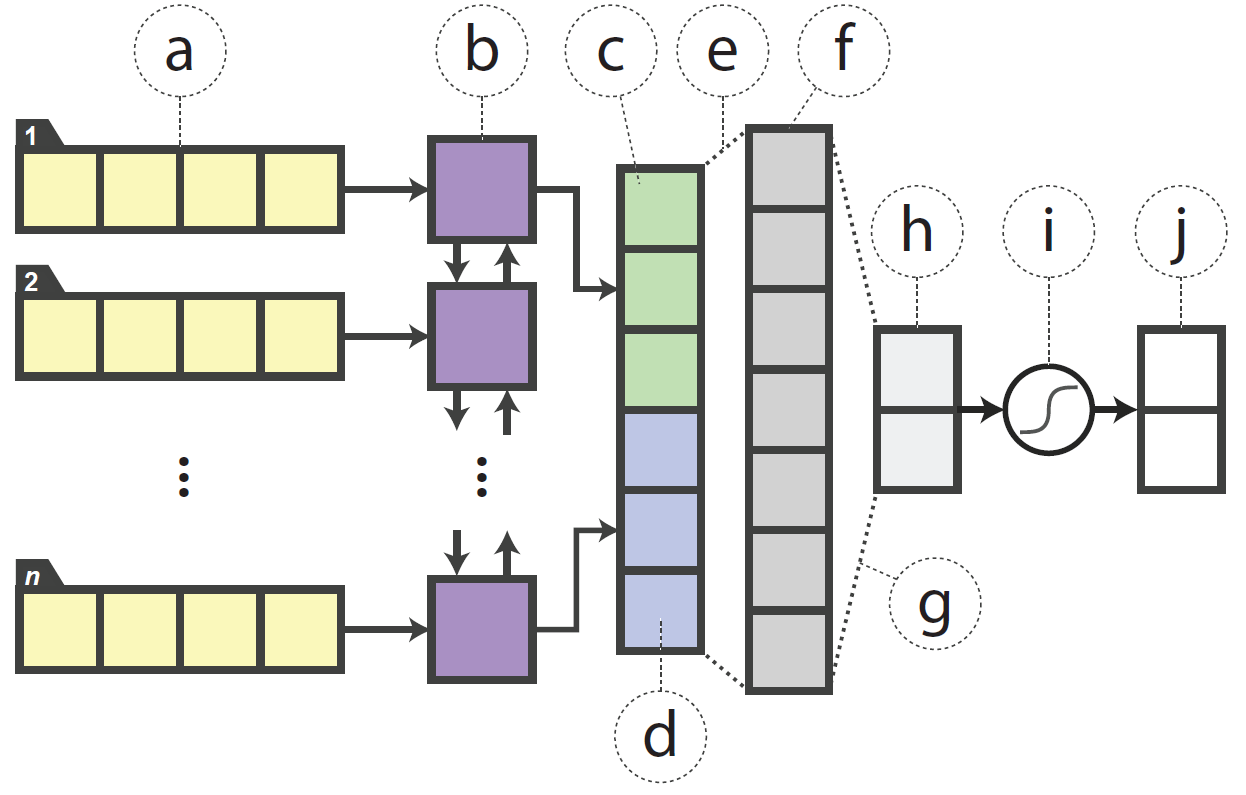
\includegraphics[width=\linewidth]{figures/05-related_work/biLSTM_tang_2019.png}
%     \caption[The BiLSTM model for single-sentence classification]{The BiLSTM model for single-sentence classification of \citet{tang2019distilling}. The labels are (a) input embeddings, (b) BiLSTM, (c, d) backward and forward hidden states, respectively, (e, g) fully-connected layer; (e) with ReLU, (f) hidden representation, (h) logit outputs, (i) softmax activation, and (j) final probabilities. Source: \citep{tang2019distilling}}
%     \label{fig:BiLSTM_tang_2019}
% \end{marginfigure}

Furthermore, instead of using the \gls{kld} of the class probability distributions of the student and teacher networks as a soft target loss, \citet{tang2019distilling} opted to penalize the \gls{mse} between the student network's logits against those of the teacher network instead:
\begin{align}
    \label{eq:mse_loss}
    \loss{\vect{z}_s, \vect{z}_t} &= \norm{\vect{z}_t - \vect{z}_s}_2^2
\end{align}


% chatterjee 2019
% \citet{chatterjee2019making} applied \gls{kd} on the end-task level for the SQuAD task  \citep{rajpurkar2016squad,rajpurkar2018know} (see \cref{subsec:SQuAD}) in order to transfer knowledge from \bertbase as fine-tuned on SQuAD to to a smaller version of BERT, which they named \bertsmall ($L=6$, $H=768$, $A=12$, $\#P=\SI{67.5}{\mega\nothing}$). Their \bertsmall was initialized from every other layer of the fine-tuned \bertbase.


% liu 2019
Much like the original work of \citet{bucil2006model}, \citet{liu2019improving} apply \gls{kd} to an ensemble of teacher networks in a \gls{mtl} setting in order to generalize the knowledge that is transferred to the student network. The authors use the \gls{mtdnn} \citep{liu2019multi} as their architecture of choice for both their teacher networks and student network\sidenote{Actually, \gls{mtdnn} is built on top of \bertlarge.}, so there is actually no ``compression'' here, as the student network is not any smaller or faster than the teacher network.
% \sidenote{Teacher networks: Ensemble of 3 \gls{mtdnn}\\Student network: \gls{mtdnn}\\Transfer dataset: fine-tuning task (GLUE)\\Loss function: \gls{ce} for both hard and soft targets\\Stage: fine-tuning}

First, they trained 6 \glspl{mtdnn} with slightly different hyperparameters, before selecting the top 3. These top-3 networks are then fine-tuned on each of four the end-tasks, to form four end-task-specific ensembles, each consisting of 3 \gls{mtdnn} teacher networks that are fine-tuned on the specific end-task itself.

Next they use a single \gls{mtdnn} as their student network, and apply \gls{kd} on the end-task level. With this set-up, the logits of the ensemble of $N$ teacher networks are given by:
\begin{align}
    \vect{z}_{\text{ensemble}} &= \frac{1}{N} \sum_{n=1}^N \vect{z}_n,
\end{align}

where $\vect{z}_n$ are the logits of the $n^{\text{th}}$ teacher network. For their soft target loss, \citet{liu2019improving} opt for the \gls{ce} (instead of the \gls{kld} or \gls{mse} we've seen previously):

\begin{align}
    \mathcal{L}_{\text{soft}} = \loss{\vect{z}_s, \vect{z}_{\text{ensemble}}} &= \ce{\softmax{\vect{z}_s}, \softmax{\vect{z}_{\text{ensemble}}}}.
\end{align}

Their overall loss function is a simple average of the hard target loss (as in \cref{eq:hard_target_loss}) and their soft target loss. They evaluate their approach on the \gls{glue} benchmark.

% yang 2019
Similarly, \citet{yang2019model} apply \gls{kd} to an ensemble of teacher networks in a \gls{stl} setting instead. The authors use \bertbase as the architecture for their teacher networks, and a smaller version of it that uses only its first three layers as their student network, which they refer to as their ``Single Student Model'' ($L=3$, $H=768$, $FF=3072$, $A=12$, $\#P=\SI{45.9}{\mega\nothing}$). Furthermore, they report using $N$ different teachers in the ensemble\sidenote{Nowhere in their work is the value of $N$ specified.}, which are all fine-tuned on the end-task using different hyperparameters.
% \sidenote{Teacher networks: Ensemble of $N$ \bertbase\\Student network: \bertbase with only 3 layers ($L=3$, $H=768$, $FF=3072$, $A=12$, $\#P=\SI{45.9}{\mega\nothing}$)\\Transfer dataset: fine-tuning task (``DeepQA'')\\Loss function: \gls{ce} for hard, average \gls{mse} for soft\\Stage: fine-tuning}

They use cross-entropy as their hard target loss (as in \cref{eq:hard_target_loss}) and a simple average of the \gls{mse} of the logits of the student network as compared to those of the teacher (as in \cref{eq:mse_loss}):
\begin{align}
    \mathcal{L} &= (1 - \alpha) \cdot \ce{\softmax{\vect{z}_s}, \vect{y}} + \frac{\alpha}{N} \sum_{n=1}^N \norm{\vect{z}_n - \vect{z}_s}_2^2,
\end{align}

where $\alpha$ is a coefficient\sidenote{Similarly, nowhere in their work is the value of $\alpha$ specified.}.

Their end-task of choice is \gls{qa}. For this, the authors use their own experimental dataset, which they call ``DeepQA''. This dataset consists of $1$M samples, where each sample consists of a question, a passage and a binary label indicating whether the question can be answered by the passage.


% sun 2019
Recognizing the saliency of the knowledge encoded in intermediate layers of Transformer-based architectures, \citet{sun2019patient} introduce \gls{pkd}, in which a student network \emph{patiently} learns from multiple intermediate layers of the teacher network for incremental knowledge extraction. In addition to the the soft target loss (as in \cref{eq:soft_target_loss_scaled}) and hard target loss (as in \cref{eq:hard_target_loss}), they define an additional loss term as the \gls{mse} between the (normalized) hidden states of the student and teacher networks:
% \sidenote{Teacher network: \bertbase\\Student networks: \bertthree ($L=3$, $H=768$, $FF = 3072$, $A=12$, $\#P=\SI{45.7}{\mega\nothing}$) and \bertsix ($L=6$, $H=768$, $FF = 3072$, $A=12$, $\#P=\SI{67.0}{\mega\nothing}$)\\Transfer dataset: fine-tuning task (GLUE)\\Loss function: \gls{ce} for hard, \gls{kld} for soft and \gls{mse} for hidden states\\Stage: fine-tuning}

\begin{align}
    \mathcal{L}_{\text{hidden state}} &= \loss{\hvect_s, \hvect_t} = \sum_{l=1}^L \norm{\frac{\hvect_s^{(l)}}{\norm{\hvect_s^{(l)}}_2} - \frac{\hvect_t^{(\text{map}(l))}}{\norm{\hvect_t^{(\text{map}(l))}}_2}}_2^2, \\
    \mathcal{L}_{\text{PKD}} &= \alpha \cdot \mathcal{L}_{\text{soft}} + (1 - \alpha) \cdot \mathcal{L}_{\text{hard}} + \beta \cdot \mathcal{L}_{\text{hidden state}},
\end{align}

where $\hvect_s$ and $\hvect_t$ are the student and teacher hidden states, respectively, $L$ denotes the number of layers in the student network, and $\text{map}(\cdot)$ defines a mapping from layers of the student network to layers of the teacher network. 

Furthermore, they use \bertbase as their teacher network (which they refer to as \berttwelve), and two smaller versions of it as their student networks: \bertthree ($L=3$, $H=768$, $FF = 3072$, $A=12$, $\#P=\SI{45.7}{\mega\nothing}$) and \bertsix ($L=6$, $H=768$, $FF = 3072$, $A=12$, $\#P=\SI{67.0}{\mega\nothing}$), which are initialized from the first 3 (respectively 6) layers of \bertbase. \gls{kd} is applied at the end-task level for a subset of the GLUE benchmark (see \cref{subsec:GLUE}), namely SST-2, MRPC, QQP, MNLI, QNLI and RTE.

Lastly, the authors experiment with two different mappings (which they call strategies):  \emph{Skip}, where the student learns from every $k^{\text{th}}$ layer of the teacher:
\begin{align*}
    \text{map}_{\text{skip}}(l) = k \cdot l,
\end{align*}

 and \emph{Last}, where the student learns from the last $k$ layers of the teacher:
 
\begin{align*}
    \text{map}_{\text{last}}(l) = l + M - (k + 1),
\end{align*}

where $M$ denotes the number of layers in the teacher network.


% jiao 2019
\citet{jiao2019tinybert} leverage not only the knowledge from the hidden states and final prediction layer, but also from the embedding layers and attention heads. To this end, they define the following loss functions:
% \sidenote{Teacher network: \bertbase\\Student networks: TinyBERT ($L=4$, $H=312$, $FF = 1200$,  $A=12$, $\#P=\SI{14.5}{\mega\nothing}$)\\Transfer dataset: ``large-scale text corpus'' for pre-training, fine-tuning task (GLUE and SQuAD) for fine-tuning\\Loss function: \gls{mse} for attention matrices, hidden states and embeddings. ``Soft'' cross-entropy for prediction layer\\Stage: both stages}
\begin{align}
    \mathcal{L}_{\text{attn}} &= \frac{1}{A} \sum_{a=1}^A \norm{\vect{A}_s^{(a)} - \vect{A}_t^{(a)}}_2^2, \\
    \label{eq:attention_mse}
    \mathcal{L}_{\text{hidn}} &= \norm{\vect{H}_s - \vect{H}_t}_2^2, \\
    \mathcal{L}_{\text{embd}} &= \norm{\vect{E}_s - \vect{E}_t}_2^2, \\
    \mathcal{L}_{\text{pred}} &= \ce{\softmax{\vect{z}_s / t}, \softmax{\vect{z}_s}},
    % \mathcal{L}_{\text{pred}} &= KL\left( \softmax{\vect{z}_s / T} || \softmax{\vect{z}_t} \right),
\end{align}

where $\vect{A}_s^{(a)}$ and $\vect{A}_t^{(a)}$ are the student and teacher attention matrices corresponding to the $a^{\text{th}}$ attention head, respectively, $\vect{H}_s$ and $\vect{H}_t$ are the student and teacher hidden states, respectively, $\vect{E}_s$ and $\vect{E}_t$ are the student and teacher embeddings, respectively, and $t$ is the temperature (\citet{jiao2019tinybert} use $t = 1$).

Using $l=0$ as the index of the embedding layer and $l = L + 1$ for the index of the prediction layer, the combined loss function is given by:
\begin{align}
    \mathcal{L}_{\text{model}} &= \sum_{l=0}^{L+1} \lambda_l \mathcal{L}_{\text{layer}} \left( S_l, T_{\text{map}(l)} \right), \\
    \mathcal{L}_{\text{layer}} \left( S_l, T_{\text{map}(l)} \right) &= \begin{cases}
        \mathcal{L}_{\text{embd}} \left( S_0, T_0 \right) & \text{if } l = 0 \\
        \mathcal{L}_{\text{hidn}} \left( S_l, T_{\text{map}(l)} \right) + \mathcal{L}_{\text{attn}} \left( S_l, T_{\text{map}(l)} \right) & \text{if } 0 < l \leq L \\
        \mathcal{L}_{\text{pred}} \left( S_{L+1}, T_{M+1} \right) & \text{if } l = L + 1
    \end{cases},
\end{align}

where $S$ refers to the student network, $T$ refers to the teacher network, $\lambda_l$ is a hyperparameter that represents the importance of the $l^{\text{th}}$ layer's distillation.

Furthermore, they introduce a two-stage distillation framework:
\begin{enumerate}
    \item General Distillation: Using a pre-trained teacher network, apply \gls{kd} during pre-training, such that the student network becomes a compact, general-purpose pre-trained \gls{lm}, which can then be fine-tuned on any given end-task.
    \item End-task-specific Distillation: Using a teacher network that is fine-tuned on the given end-task, apply \gls{kd} during fine-tuning, such that the student network becomes a compact, fine-tuned \gls{lm} that is specialized in the given end-task.
\end{enumerate}

In their work, they use \bertbase as their teacher network and a ``tiny'' Transformer which they call TinyBert as their student network ($L=4$, $H=312$, $FF = 1200$,  $A=12$, $\#P=\SI{14.5}{\mega\nothing}$). During their ``General Distillation'', they use a ``large-scale text corpus''\sidenote{Nowhere in their work is the actual composition of this corpus specified} for their transfer dataset. TinyBERT is further fine-tuned and evaluated on the GLUE benchmark (see \cref{subsec:GLUE}).

% turc 2019
\citet{turc2019well} separate the \gls{kd} process from either pre-training or fine-tuning. Instead, they first pre-train their student network (a smaller version of BERT) using the \gls{mlm} and \gls{nsp} objectives before performing end-task-specific \gls{kd} using only a soft target loss (followed by optional fine-tuning with a hard target loss). They call their method \gls{pd}.
% \sidenote{Teacher network: \bertbase (and \bertlarge)\\Student networks: 24 different network sizes, ranging from their Transformer$_{\text{TINY}}$ ($L=2$, $H=128$, $FF=512$, $A=2$, $\#P=\SI{4.4}{\mega\nothing}$) to their Transformer$_{\text{BASE}}$ ($L=12$, $H=768$, $FF=3072$, $A=12$, $\#P=\SI{110.1}{\mega\nothing}$)\\Transfer dataset: \gls{tbc} + English Wikipedia for pre-training, task-specific for \gls{kd}\\Loss function: a lot \\Stage: fine-tuning (no KD during pre-training)}

Like \citet{devlin2018bert}, \citet{turc2019well} use a concatenation of the \gls{tbc} and English Wikipedia as their pre-training corpus. After pre-training, they perform \gls{kd} using unlabeled data ($\dataset_T$), after which evaluation is performed using labeled data ($\dataset_L$) for various tasks.

They performed experiments with 24 different student network sizes, ranging from their Transformer$_{\text{TINY}}$ ($L=2$, $H=128$, $FF=512$, $A=2$, $\#P=\SI{4.4}{\mega\nothing}$) to their Transformer$_{\text{BASE}}$ ($L=12$, $H=768$, $FF=3072$, $A=12$, $\#P=\SI{110.1}{\mega\nothing}$), which has the exact same architecture and size as \bertbase. In their experiments, they used both \bertbase and \bertlarge as their teacher network. Their approach was evaluated on a subset of the \gls{glue} benchmark, namely: SST-2, MRPC, QQP, MNLI, QNLI and RTE (see \cref{subsec:GLUE}).


% sanh 2019
\citet{sanh2019distilbert} opt for a \emph{cosine embedding loss} in order to leverage the knowledge in the intermediate layers, which uses the cosine distance:
\begin{align}
    \label{eq:cosine_embedding_loss}
    \mathcal{L}_{\text{cos}} &= \loss{\hvect_s, \hvect_t} = 1 - \cos{\left( \hvect_s, \hvect_t \right)}, \\
    \mathcal{L} &= \alpha_1 \cdot \mathcal{L}_{\text{soft}} + \alpha_2 \cdot \mathcal{L}_{\text{hard}} + \alpha_3 \cdot \mathcal{L}_{\text{cos}},
\end{align}
where $\alpha_1 = \alpha_2 = \alpha_3 = \frac{1}{3}$. 

They use \bertbase as their teacher network, and a smaller version of it as their student network, which they call DistilBERT ($L=6$, $H=768$, $FF = 3072$, $A=12$, $\#P=\SI{66.4}{\mega\nothing}$), which is initialized from the $1^{\text{st}}$, $3^{\text{rd}}$, $5^{\text{th}}$, $8^{\text{th}}$, $10^{\text{th}}$, and $12^{\text{th}}$ layers of \bertbase, respectively\sidenote{Nowhere in their work do they specify which exact layers from \bertbase they used for the initialization of their DistilBERT. We only learned this after correspondence with the authors.}.
% \sidenote{Teacher network: \bertbase\\Student network: DistilBERT ($L=6$, $H=768$, $FF = 3072$, $A=12$, $\#P=\SI{66.4}{\mega\nothing}$)\\Transfer dataset: \gls{tbc} + English Wikipedia\\Loss function: \gls{ce} for hard targets, \gls{kld} for soft targets, cos for the hidden states.\\Stage: pre-training}

The authors apply \gls{kd} during pre-training with the \gls{mlm} objective, such that the student network becomes a compact, general-purpose pre-trained \gls{lm}, which can then be fine-tuned on any given end-task.

They evaluate their DistilBERT on both the \gls{glue} benchmark (see \cref{subsec:GLUE}) and \gls{squad} (see \cref{subsec:SQuAD}) in order to assess the downstream task performance of their general-purpose pre-trained \gls{lm}.


% sun 2020
Similar to \citet{sanh2019distilbert}, \citet{sun2020mobilebert} apply \gls{kd} during pre-training, such that the resulting student network is a compact, ``task-agnostic'', general-purpose \gls{lm}, which they call MobileBERT. In their set-up, they used a (significantly) modified version of \bertlarge (which they refer to as ``Inverse Bottleneck'' \bertlarge or IB-\bertlarge for short) as their teacher network and a deep, but thin copy of it as their student network, which they call MobileBERT.
% \sidenote{Teacher network: IB-\bertlarge ($\#P=\SI{293}{\mega\nothing}$) \\Student network: MobileBERT ($\#P=\SI{25.3}{\mega\nothing}$)\\Transfer dataset: \gls{tbc} + English Wikipedia\\Loss function: a lot\\Stage: pre-training}

This is different from most approaches discussed previously, where the student network is effectively a more shallow version of the teacher network (i.e. the same hidden size $H$, feed-forward size $FF$ and number of self-attention heads $A$, but a smaller number of layers $L$). Instead, their teacher and student networks boast the same number of layers, but different hidden and feed-forward sizes.

The authors further define a layer-wise knowledge transfer loss $\mathcal{L}^{\ell}_{KT}$ for every $\ell^\text{th}$ layer that is very similar to that of \citet{jiao2019tinybert}, which is a linear combination of a hidden layer loss $ \mathcal{L}_{\text{hidn}}$ (which they call \gls{fmt}) and an attention head loss $ \mathcal{L}_{\text{attn}}$ (which they call \gls{at}).

In fact, the hidden layer loss $\mathcal{L}_{\text{hidn}}$ is exactly the same as in \cref{eq:attention_mse}, whereas for the attention head loss, \citet{sun2020mobilebert} use the \gls{kld} between the attention heads instead of the \gls{mse}:
\begin{align}
    \mathcal{L}_{\text{attn}} &= \frac{1}{A} \sum_{a=1}^A KL\left( \vect{A}_s^{(a)} || \vect{A}_t^{(a)} \right),
\end{align}

where $\vect{A}_s^{(a)}$ and $\vect{A}_t^{(a)}$ are the student and teacher attention matrices corresponding to the $a^{\text{th}}$ attention head.

Next to this layer-wise knowledge transfer loss, the authors define their \gls{pd_sun} loss as a (sort of) linear combination of the \gls{mlm} loss $\mathcal{L}_{MLM}$, the \gls{nsp} loss $\mathcal{L}_{NSP}$ and a \gls{kd} loss $\mathcal{L}_{KD}$:
\begin{align}
    \mathcal{L}_{PD} &= \alpha \cdot \mathcal{L}_{MLM} + (1 - \alpha) \cdot \mathcal{L}_{KD} + \mathcal{L}_{NSP}.
\end{align}

Following the example of \citet{devlin2018bert}, the authors use a concatenation of the \gls{tbc} and English Wikipedia as their pre-training corpus. Like \citet{sanh2019distilbert}, \citet{sun2020mobilebert} evaluate the downstream task performance of their MobileBERT on both the \gls{glue} benchmark (see \cref{subsec:GLUE}) and \gls{squad} (see \cref{subsec:SQuAD}).

As a service to the reader, the various papers discussed in this chapter have been summarized in \cref{tab:related_works_summary}.

\begin{landscape}
    \advance\vsize6cm
    \csname @colroom\endcsname=\vsize
    \textheight=\vsize
    \csname @colht\endcsname=\vsize
    \renewcommand*{\arraystretch}{1.4}
    \small
    \begin{longtable}{l | l c l l c c c c l }
        \caption[Summary of related works]{Summary of related works along the questions posed at the start of this chapter. ``FT'' stands for fine-tuning, whereas ``PT'' denotes pre-training, and ``EnWiki'' refers to English Wikipedia.}
        \label{tab:related_works_summary}\\
        \toprule
        \B{Paper} & \B{Teacher network} & \B{Ensemble?} & \B{Student network(s)} & \B{Stage} & \B{Pre-training dataset} & \B{$\mathcal{L}_{\text{soft}}$} & \B{$\mathcal{L}_{\text{hard}}$} & \B{$\mathcal{L}_{\text{hidden}}$} & \B{Evaluation} \\
        \midrule
        \citet{tang2019distilling} & \bertlarge & \redtimes & \gls{bilstm} & FT & \redtimes & \gls{mse} & \gls{ce} & \redtimes & Subset of \gls{glue}  \\
        \citet{liu2019improving} & \gls{mtdnn} & \greencheck & \gls{mtdnn} & FT & \redtimes & \gls{ce} & \gls{ce} & \redtimes & \gls{glue} \\
        \citet{yang2019model} & \bertbase & \greencheck & \bertthree & FT & \redtimes & \gls{kld} & \gls{ce} & \redtimes & DeepQA \\
        \citet{sun2019patient} & \bertbase & \redtimes & \bertthree \& \bertsix & FT & \redtimes & \gls{kld} & \gls{ce} & \gls{mse} & Subset of \gls{glue} \\
        \citet{jiao2019tinybert} & \bertbase & \redtimes & TinyBERT & Both & ``large-scale text corpus'' & \gls{ce} & \redtimes & \gls{mse} & \gls{glue} \\
        \citet{turc2019well} & \bertbase \& \bertlarge & \redtimes & Various sizes & FT & \gls{tbc} + EnWiki & \gls{ce} & \redtimes & \redtimes & Subset of \gls{glue} \\
        \citet{sanh2019distilbert} & \bertbase & \redtimes & DistilBERT & PT & \gls{tbc} + EnWiki & \gls{kld} & \gls{ce} & Cosine distance & \gls{glue} \& \gls{squad} \\
        \citet{sun2020mobilebert} & IB-\bertlarge & \redtimes & MobileBERT & PT & \gls{tbc} + EnWiki & \gls{kld} & \gls{ce} & \gls{mse} & \gls{glue} \& \gls{squad} \\
        \bottomrule
    \end{longtable}
\end{landscape}